\section{Conceptos fundamentales de la teor\'ia cin\'etica y transporte en el Plasma}

  Los gases ionizados pueden ser espec\'ificados por una funci\'on de distribuci\'on $f_\alpha$(\textbf{r}, \textbf{v}, t). Una derivaci\'on Eur\'istica lleva a la conocida ecuaci\'on cin\'etica\cite{freidberg2014} 

  \begin{equation}\label{eq:k}
    \frac{df_\alpha}{dt} \equiv \left(\partial_t + \textbf{v}\cdot\nabla + \frac{Z_\alpha e}{m_\alpha}(\textbf{E} + \textbf{v}\times\textbf{B})\cdot \nabla_\textbf{v} \right)f_\alpha = C_\alpha
  \end{equation}

  \textbf{Esta ecuaci\'on no toma en cuenta fluctuaciones termicas}. Representa densidades suaves promediadas sobre un volumen con un gran n\'umero de part\'iculas. Los campos $\textbf{E}$ y $\textbf{B}$ tambi\'en varian suavemente, no hay fluctuaciones r\'apidas de microcampos y microfuerzas. Dichos efectos se consideran solo en el t\'ermino de colisiones $C_\alpha$.

  Ahora de la mec\'anica est\'istica es posible obtener los momentos de una distribuci\'on, nos interesa el primer y segundo momento\cite{helander2005} de la distribuci\'on definidos como 

  \begin{eqnarray}
    n_\alpha &=& \int d^3v f_\alpha \label{eq:dens}\\
    \textbf{u}_{\alpha} &=& \frac{1}{n_\alpha}\int d^3v f_\alpha\textbf{v} \label{eq:vel} \\
    \textbf{Q}_\alpha &\equiv& \frac{m_\alpha n_\alpha \left<v^2\textbf{v}\right>}{2}\label{eq:heat}
  \end{eqnarray}

El momento cero en la Ec. \eqref{eq:dens} es la densidad de part\'iculas de una especie en el plasma, i.e., el n\'umero de part\'iculas de una especie por unidad de volumen. El primer momento Ec.\eqref{eq:vel} es la velocidad promedio de las part\'iculas de una especie en el plasma. La Ec.\eqref{eq:heat} es el flujo de energ\'ia. 

  Ahora definimos el flujo de part\'iculas en el plasma como 
  
  \begin{equation}
    \pmb{\Gamma}_\alpha \equiv n_\alpha\textbf{u}_\alpha
  \end{equation}

  De la ecuaci\'on cin\'etica \eqref{eq:k}, es posible obtener la siguiente ecuaci\'on de continuidad

  \begin{equation}\label{eq:cont}
    \partial_t n_\alpha + \nabla\cdot\pmb{\Gamma}_\alpha = S_\alpha
  \end{equation}

  donde $S_\alpha$ son las fuentes y/o sumideros de las part\'iculas $\alpha$. En estado estacionario como sugiere \cite{lechte2002} la Eq. \eqref{eq:cont} se reduce a 

  \begin{eqnarray*}
    \nabla\cdot\pmb{\Gamma}_\alpha = S_\alpha \\
    \implies \int_V d^3r\nabla\cdot\pmb{\Gamma}_\alpha = \int_V d^3r S_\alpha\\
    \implies \oint_{\partial V} \pmb{\Gamma}_\alpha\cdot d\textbf{S} = \int_V d^3r S_\alpha
  \end{eqnarray*}

  Definimos el flujo radial de part\'iculas como

  \begin{equation}\label{eq:rtpf}
    \Gamma_n^\alpha \equiv \oint_{\partial V} \pmb{\Gamma}_\alpha \cdot d\textbf{S} = \int_V d^3r S \approx \left<S\right>V
  \end{equation}

  Como es visible al adentrarse en balances globales, el concepto de promedios superficiales es fundamental. Conocer todos los parametros del plasma en su superficie ser\'a la piedra angular de los modelos que estamos por desarrollar.

  \begin{shaded}
    \textbf{Promedio Superficial}

    Definimos el promedio de una cantidad vectorial en la superficie como 

    \begin{equation}
      \left<\pmb{\varDelta}\right>_{\partial V} \equiv \frac{1}{A}\oint_{\partial V}\pmb{\varDelta}\cdot d\textbf{S}
    \end{equation}

    donde $A$ es el \'area superficial del plasma.
  \end{shaded}

  de lo anterior, podemos ver que el flujo radial de part\'iculas es simplemente el promedio superficial del flujo de part\'iculas que atraviesan la superficie, i.e., $\Gamma_n^\alpha = A\left<\Gamma_\alpha\right>_{\partial V}$ \cite{dinklage2005}.
  
  Ahora a partir de la llamada ecuaci\'on de energ\'ia \cite{helander2005} derivada de la Eq. \eqref{eq:k} se tiene que

  \begin{equation}\label{eq:energy}
    \frac{\partial}{\partial t}\left(\frac{3n_\alpha T_\alpha}{2} + \frac{m_\alpha n_\alpha u_\alpha^2}{2}\right) + \nabla\cdot\textbf{Q} = Z_\alpha e n_\alpha \textbf{E}\cdot\textbf{u}_\alpha + \int d^3v\frac{mv^2}{2}C_\alpha
  \end{equation} 

  En el lado izquierda de la Ec.\eqref{eq:energy} el primer t\'ermino corresponde al calentamiento de Joule en el plasma, para explicar el segundo se debe introducir los siguientes t\'erminos

  \begin{eqnarray}
    \textbf{w}_\alpha &\equiv& \textbf{v} - \textbf{u}_\alpha \nonumber\\
    \textbf{R}_\alpha &\equiv& \int d^3v m_\alpha\textbf{v}C_\alpha \nonumber\\
    \mathcal{Q}_\alpha &\equiv& \int d^3v \frac{mw_\alpha^2}{2}C_\alpha \nonumber\\
    \frac{3}{2}T_\alpha &\equiv& \left<\frac{m_\alpha w^2}{2}\right> \label{eq:temp}
  \end{eqnarray}

  Cada una de ellas corresponde a:
  \begin{itemize}
    \item $\textbf{w}_\alpha$ : desviaci\'on de la velocidad de la part\'icula de la velocidad promedio, i.e., velocidad por movimiento aleatorio. Cumple que $\left<\textbf{w}_\alpha\right> = \textbf{0}$.
    \item $\textbf{R}_\alpha$ : fuerza ejercida en la part\'icula como resultado de la colisi\'on con otras especies en el plasma.
    \item $\mathcal{Q}_\alpha$ : raz\'on de la energ\'ia t\'ermica transferida por colisiones con otras especies. 
  \end{itemize}

  El segundo t\'ermino en el lado izquierdo de la Ec.\eqref{eq:energy} es entonces, \textbf{la energ\'ia total transferida} por colisiones con otras especies.

  \begin{equation}
     \int d^3v \frac{m_\alpha v^2}{2}C_\alpha = \mathcal{Q}_\alpha + \textbf{R}_\alpha\cdot\textbf{u}_\alpha
  \end{equation}

  Aqu\'i el t\'ermino $\textbf{R}_\alpha\cdot\textbf{u}_\alpha$ corresponde al trabajo por unidad de tiempo realizado por la fuerza $\textbf{R}_\alpha$.

  B\'asicamente el lado izquierdo de la ecuaci\'on es la potencia debido al calentamiento de Joule o por colisiones con otras part\'iculas. En el caso estacionario la Ec. \eqref{eq:energy} se vuelve

  \begin{eqnarray}
  \nabla\cdot\textbf{Q} = \mathcal{Q}_\alpha + (Z_\alpha e n_\alpha\textbf{E} + \textbf{R}_\alpha)\cdot\textbf{u}_\alpha \nonumber\\
    \int_V d^3r \nabla\cdot\textbf{Q} = \mathcal{Q}_\alpha + (Z_\alpha e n_\alpha\textbf{E} + \textbf{R}_\alpha)\cdot\textbf{u}_\alpha\nonumber\\
    \oint_{\partial V} \textbf{Q}\cdot d\textbf{S} = \int_V d^3r\left[\mathcal{Q}_\alpha + (Z_\alpha e n_\alpha\textbf{E} + \textbf{R}_\alpha)\cdot\textbf{u}_\alpha\right] \nonumber
    \end{eqnarray}

    Finalmente llegamos a la siguiente expresi\'on al definir el flujo radial de energ\'ia $\Gamma_E \equiv \oint_{\partial V} \textbf{Q}\cdot d\textbf{S}$ y $Q \equiv \mathcal{Q}_\alpha + (Z_\alpha e n_\alpha\textbf{E} + \textbf{R}_\alpha)\cdot\textbf{u}_\alpha$.

    \begin{equation}
      \Gamma_E = \int_Vd^3r Q \approx \left<Q\right>V
    \end{equation}

   Trabajaremos con estas definiciones m\'as adelante.

   \subsection{Procesos de calentemiento en el Plasma}

  Hasta el momento no se han hecho muchas consideraciones sobre el Plasma con el que se esta trabajando. Ahora para el modelo en estudio imponemos la condici\'on de un confinamiento en el r\'egimen de transporte cl\'asico. Esto es, los flujos de part\'iculas y energ\'ia obdecen la ley de Fick's es decir los flujos de part\'iculas y energ\'ia pueden ser descritos mediante los gradientes de densidad $n_\alpha$ y temperatura $T_\alpha$ en casos donde el campo $\textbf{B}$ es uniforme.

  Por lo pronto dejaremos de lado los sub\'indices. Retomemos el estudio de la cantidad $\textbf{Q}$ que estudiamos en la secci\'on anterior, y añadamos las siguientes definiciones

  \begin{eqnarray}
    \textbf{q} &\equiv& \frac{1}{2}mn\left<w^2\textbf{w}\right>\label{eq:q} \\
    \textbf{P} &\equiv&  mn\left<\textbf{ww}\right>\label{eq:tensorP} \\
    p &\equiv& \frac{1}{3}Tr(\textbf{P}) = \frac{1}{3}mn\left<w^2\right> \label{eq:pressureanisotropic}
  \end{eqnarray}

  Ahora profundizamos m\'as en los flujos de calor y las diferentes formas en las que la energ\'ia se difunde en el plasma. Comencemos partiendo de lo siguiente

  \begin{eqnarray*}
    \left<w^2\textbf{w}\right> = \left<(\textbf{v} - \textbf{u})\cdot(\textbf{v} - \textbf{u})\left[\textbf{v} - \textbf{u}\right]\right> \\
    = \left<(v^2 + u^2 - 2\textbf{u}\cdot\textbf{v})\left[\textbf{v}-\textbf{u}\right]\right> \\
    = \left< v^2\textbf{v} + u^2\textbf{v} - 2(\textbf{u}\cdot\textbf{v})\textbf{v} - v^2\textbf{u} - u^2\textbf{u} + 2(\textbf{u}\cdot\textbf{v})\textbf{u}\right>\\
    = \left<v^2\textbf{v}\right> + u^2\left<\textbf{v}\right> - u^2\textbf{u} - \left<v^2\right>\textbf{u} - 2\textbf{u}\cdot\left<\textbf{vv}\right> + 2\textbf{u}\cdot\left<\textbf{vu}\right>\\
    = \left<v^2\textbf{v}\right> + \cancel{u^2\textbf{u}} - \cancel{u^2\textbf{u}} - \left<v^2\right>\textbf{u} - 2\textbf{u}\cdot\left<\textbf{vv}\right> + 2\textbf{u}\cdot\left<\textbf{vu}\right>\\
    = \left<v^2\textbf{v}\right> -\left<v^2\right>\textbf{u} - 2\textbf{u}\cdot\left<\textbf{vv}\right> + 2\textbf{u}\cdot\left<\textbf{vu}\right>
  \end{eqnarray*}

  Ahora multiplicamos ambos lados de la ecuaci\'on por un factor de $\frac{1}{2}mn$ lo que resulta, usando las definiciones anteriores 
  
  \begin{eqnarray*}
    \textbf{q} = \textbf{Q} - \frac{1}{2}mn\left<v^2\right>\textbf{u} - mn\textbf{u}\cdot[\left<\textbf{vv} - \textbf{vu}\right>]
  \end{eqnarray*}


  \begin{shaded}
  
    Usaremos el siguiente resultado para simplificar m\'as la relaci\'on
    
    \begin{eqnarray*}
      \textbf{u}\cdot\left<\textbf{ww}\right> = \textbf{u}\cdot\left<(\textbf{v} - \textbf{u})(\textbf{v} - \textbf{u})\right>\\
      = \textbf{u}\cdot(\left<\textbf{vv}\right> + \left<\textbf{uu}\right> - \left<\textbf{uv}\right> - \left<\textbf{vu}\right>) \\
      = \textbf{u}\cdot\left<\textbf{vv}\right> + \cancel{u^2\textbf{u}} - \cancel{u^2\textbf{u}} - \textbf{u}\cdot\left<\textbf{vu}\right>\\
      = \textbf{u}\cdot[\left<\textbf{vv}\right> - \left<\textbf{vu}\right>]
    \end{eqnarray*}

    Tambi\'en usaremos el siguiente resultado

    \begin{eqnarray*}
      \left<w^2\right> = \left<v^2 + u^2 - 2\textbf{u}\cdot\textbf{v}\right>\\
      = \left<v^2\right> + u^2 - 2\textbf{u}\cdot\left<\textbf{v}\right>\\
      = \left<v^2\right> - u^2
    \end{eqnarray*}
  \end{shaded}

  De all\'i es f\'acil ver que 

  \begin{eqnarray}
    \textbf{q} &=& \textbf{Q} -\frac{1}{2}mnu^2 - \frac{1}{2}mn\left<w^2\right> - \textbf{u}\cdot\textbf{P}\nonumber\\
    \implies \textbf{Q} &=& \textbf{q} + \frac{3}{2}Tn\textbf{u} - \frac{1}{2}mnu^2\textbf{u} - \textbf{P}\cdot\textbf{u}\nonumber \\
                        &=& \textbf{q} + \frac{3}{2}T\pmb{\Gamma} - \frac{1}{2}mu^2\pmb{\Gamma} - \textbf{P}\cdot\textbf{u}
  \end{eqnarray}

  N\'otese que por construcci\'on del tensor $\textbf{P}$ este es anisotr\'opico, sin embargo, es diagonal y las contracciones $\textbf{u}\cdot\textbf{P}$ y $\textbf{P}\cdot\textbf{u}$ son equivalentes. Una forma alternativa de ver esto se logra con el tensor $\Pi_{ij} = P_{ij} - p\delta_{ij}$ y usando $p = nT$ 

  \begin{equation}
    Q_j = q_j + \frac{5}{2}pu_j + \Pi_{jk}u_k + \frac{1}{2}mu^2\Gamma_j
  \end{equation}

  Se tienen los siguientes calentamientos en el plasma\cite{helander2005}

  \begin{itemize}
    \item $\textbf{q}$ : flujo de calentamiento conductivo.
    \item $\frac{5}{2}p\textbf{u}$ : flujo de calentamiento convectivo.
    \item $\pmb{\Pi}\cdot\textbf{u}$ : transporte viscoso de energ\'ia.
    \item $\frac{1}{2}mu^2\pmb{\Gamma}$ : convecci\'on de energ\'ia cin\'etica.
  \end{itemize}

Ahora bien, para un transporte en el cual la velocidad del flujo $\textbf{u}$ surge en respuesta a gradientes suaves ($\delta << 1$) se puede asumir que est\'a cantidad es pequeña, $u \sim \delta v_T \ll v_T$ por lo que la podemos despreciar, a la vez, si las velocidad del flujo es negligible, tambi\'en podemos asumir que el transporte viscoso de energ\'ia es pequeño en comparaci\'on a la conducci\'on y convecci\'on. Bajo estos supuestos\cite{dinklage2005}

  \begin{equation*}
    Q_j \approx q_j + \frac{5}{2}T\Gamma_j
  \end{equation*}

  De lo anterior el flujo de energ\'ia $\Gamma_E$ es dada por 

  \begin{equation}\label{eq:heatfluxp}
    \Gamma_E \approx A\left<\textbf{q}\right>_{\partial V} + A\frac{5}{2}\left<T\pmb{\Gamma}\right>_{\partial V}
  \end{equation}


   \subsection{Transporte radial y las leyes de Fick}

A partir de ahora trabajaremos con los electrones en el plasma y dejaremos de lado los sub\'indices. De momento, bajo un transporte cl\'asico donde el campo magn\'etico es homogeneo asumimos que las leyes de Fick se sostienen tal que $q_j = -\chi_{jk}\partial_k T$ y $\Gamma_j = -D_{jk}\partial_k n$, m\'as adelante justificaremos esto. La configuraci\'on del modelo es como se ve en la figura \label{fig:pgeom}. 

\begin{figure}[htb!]\label{fig:pgeom}
		\centering
		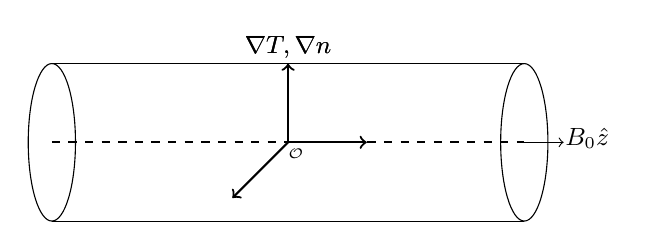
\begin{tikzpicture}[scale=1]
			% Cylinder axis from left to right
			(0,0) ellipse (0.3 and 1) % left cap
			(6,0) ellipse (0.3 and 1); % right cap (hidden)
			% Body
			(0,1) -- (6,1) arc (90:-90:1 and 0.3) -- (0,-1) arc (-90:90:1 and 0.3);
			% Front and back ellipses
			\draw (0,0) ellipse (0.3 and 1);
			\draw (6,0) ellipse (0.3 and 1);
			\foreach \angle in {0,90, 225}{
				\draw[->,thick] (3,0) -- ++(\angle:1);
			}\foreach \angle in {0,90}{
				\node at (3,1.2) {\small{$\nabla T, \nabla n$}} ++(\angle:1);
			}
			\node at (3.1,-0.15) {\tiny{$\mathcal{O}$}};
			% Cylinder outline
			\draw (0,1) -- (6,1);
			\draw (0,-1) -- (6,-1);
			\draw[dashed, thick] (0.0,0.0) -- (6.0,0.0);
			\draw[->] (6.0,0.0) -- (6.5,0.0);
			\node at (6.8,0.05) {\small{$B_0\hat{z}$}};
		\end{tikzpicture}
		\caption{Plasma Cil\'indrico con campo uniforme y transporte radial de part\'iculas y energ\'ia}
	\end{figure}

Se pueden ver que finalmente las relaciones de transporte radial, o flujo de part\'iculas y energ\'ia se pueden escribir como

  \begin{eqnarray}
    \Gamma_n &=& -A\left<\textbf{D}\cdot\nabla n\right>_{\partial V} \label{eq:partflux}\\
    \Gamma_E &=& -A\left<\pmb{\chi}\cdot\nabla T\right>_{\partial V} + \frac{3}{2}A\left<T\pmb{\Gamma}\right>_{\partial V}\label{eq:energyflux}
    \end{eqnarray}
    
  Las cantidades $\chi$ y $D$ deben ser estudiadas m\'as a fondo antes de asumir que son simplemente coeficientes, ya que podr\'an depender de la densidad $n$ y la temperatura $T$.

